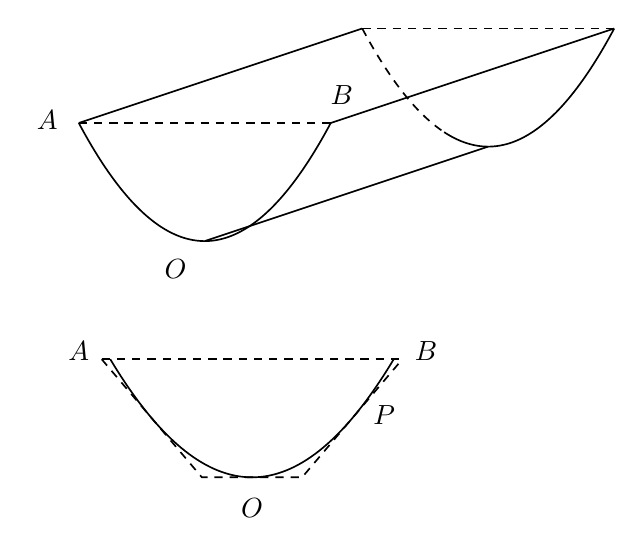
\begin{tikzpicture}[x=1cm,y=1cm,line width=.6pt,font=\normalsize,>=stealth,
  solid edge/.style={solid,line width=.6pt},
  hidden edge/.style={dashed,line width=.6pt,dash pattern=on 3pt off 2.5pt}]
% upper 3D trough
\coordinate (Af) at (0.0,4.5);
\coordinate (Of) at (1.6,3.0);
\coordinate (Bf) at (3.2,4.5);
\coordinate (Ab) at (3.6,5.7);
\coordinate (Ob) at (5.2,4.2);
\coordinate (Bb) at (6.8,5.7);
\draw[solid edge,domain=-1:1,samples=80] plot ({\x*1.6+1.6},{\x*\x*1.5+3.0});
\draw[solid edge,domain=-0.35:1,samples=60] plot ({\x*1.6+5.2},{\x*\x*1.5+4.2});
\draw[hidden edge,domain=-1:-0.35,samples=30] plot ({\x*1.6+5.2},{\x*\x*1.5+4.2});
\draw[solid edge] (Af)--(Ab);
\draw[solid edge] (Bf)--(Bb);
\draw[solid edge] (Of)--(Ob);
\draw[hidden edge] (Af)--(Bf);
\draw[hidden edge] (Ab)--(Bb);
\node[left,xshift=-4pt,yshift=1pt] at (Af) {$A$};
\node[above,xshift=4pt,yshift=3pt] at (Bf) {$B$};
\node[below left,xshift=-3pt,yshift=-3pt] at (Of) {$O$};
% lower cross-section: parabola y=1.5x^2, ground y=1.5, tangent trapezoid
\begin{scope}[shift={(0.4,0)}]
\coordinate (Al) at (0.0,1.5);
\coordinate (Br) at (3.6,1.5);
\coordinate (Ol) at (1.8,0.0);
\coordinate (Cl) at (1.1636038969,0.0000000000);
\coordinate (Cr) at (2.4363961031,0.0000000000);
\coordinate (Dl) at (-0.1091883092,1.5000000000);
\coordinate (Dr) at (3.7091883092,1.5000000000);
\coordinate (Pp) at (3.0727922061,0.7500000000);
\draw[hidden edge] (Dl)--(Dr);
\draw[solid edge,domain=-1:1,samples=80] plot ({\x*1.8+1.8},{\x*\x*1.5});
\draw[hidden edge] (Dl)--(Cl)--(Cr)--(Dr);
\node[left,xshift=-4pt,yshift=3pt] at (Al) {$A$};
\node[right,xshift=4pt,yshift=3pt] at (Br) {$B$};
\node[below,xshift=0pt,yshift=-4pt] at (Ol) {$O$};
\node[right,xshift=4pt,yshift=1pt] at (Pp) {$P$};
% no marker at P per original
\end{scope}
\end{tikzpicture}
